\documentclass[a4paper,12pt]{article}
\usepackage{../packages/coursCollege}
\newcommand{\Chapitre}{Calcul différentiel}
\renewcommand{\path}{../}
\usepackage[    %backend=biber, 
    natbib=true,
    style=numeric,
    sorting=none]{biblatex}  % Load biblatex for bibliography handling
\addbibresource{biblio-der.bib}  
\renewcommand\refname{Sources}
\renewcommand{\cours}{3MA1~--~EG~--~ns~--~2025-2026}
\usepackage{subcaption}
% Définition des couleurs
\definecolor{functioncolor}{RGB}{220,50,47}
\definecolor{tangentcolor}{RGB}{220,50,47}
\definecolor{secantcolor}{RGB}{38,139,210}
\definecolor{pointcolor}{RGB}{220,50,47}

\begin{document}
\tocloftpagestyle{fancy}
% Reduce space between section entries
\setlength{\cftbeforesecskip}{2pt}

% Reduce indentation for section entries
\setlength{\cftsecindent}{1em}
\begin{center}
{\bfseries \Huge Chapitre 2~: \\Calcul différentiel -- Partie 1}
\vspace{1cm}

\begin{tikzpicture}
% Background image
\node[inner sep=0] at (0,0) {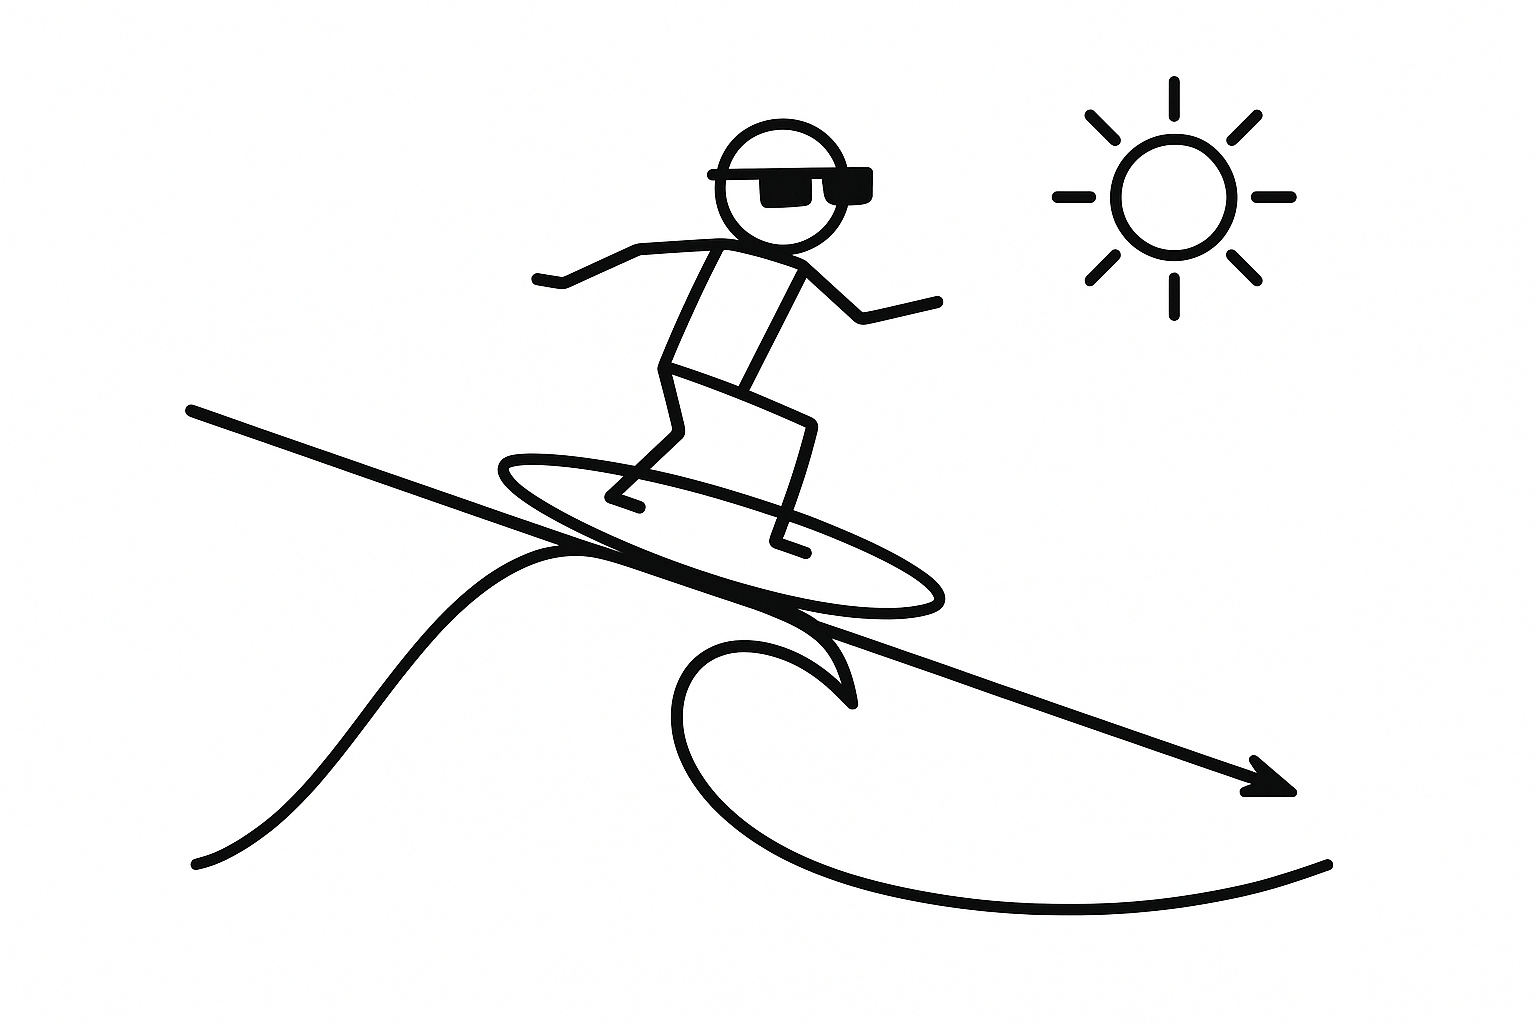
\includegraphics[width=15cm]{../medias/3M/derivation/intro}};
\end{tikzpicture}
\end{center}\vspace{-1cm}
\tableofcontents

\newpage

\subsection{Concavité et points d'inflexion}
\subsection{Application à l'étude de fonctions}

\subsection{Applications}


\subsection{Exercices}

\insertexo{g4sjk}{true}{exo}
\insertexo{d4c88}{true}{exo}
\subsubsection{Le théorème des accroissement finis}
\insertexo{d4c88}{true}{exo}
\insertexo{aef2y}{true}{exo}
\insertexo{n67du}{true}{exo}
\insertexo{5hev4}{true}{exo}
\insertexo{hju27}{true}{exo}
\insertexo{zar8b}{true}{exo}
\insertexo{x5ny2}{true}{exo}
\insertexo{r9x4h}{true}{exo}
\insertexo{147ae}{false}{exo}
\insertexo{kafhh}{false}{exo}
\insertexo{4qat4}{false}{exo}
\insertexo{qr5rf}{false}{exo}
\insertexo{7nemv}{false}{exo}
\insertexo{bw6xm}{false}{exo}
\insertexo{3m62m}{false}{exo}
\insertexo{8bwde}{false}{exo}
\insertexo{pjez7}{false}{exo}
\insertexo{c61qc}{false}{exo}
\insertexo{n67du}{true}{exo}

\subsubsection{Fonctions croissantes et décroissantes}
\insertexo{5pyfw}{false}{exo}

\subsubsection{Maximum et minimum}
\insertexo{5ab1m}{false}{exo}
\insertexo{fxy4n}{false}{exo}


\subsubsection{Optimisation}
\insertexo{ddm8s}{false}{exo}
\insertexo{sgvqw}{false}{exo}
\insertexo{tnh2w}{false}{exo}
\insertexo{rqexr}{false}{exo}
\insertexo{h6e65}{false}{exo}
\insertexo{fadzs}{false}{exo}
\insertexo{8csxg}{false}{exo}
\insertexo{js1pf}{false}{exo}
\insertexo{fydq8}{false}{exo}
\insertexo{5yxjm}{false}{exo}
\insertexo{nsmhh}{false}{exo}
\insertexo{74119}{false}{exo}
\insertexo{b52kh}{false}{exo}
\insertexo{j8hdu}{false}{exo}
\insertexo{ju1wa}{false}{exo}
\insertexo{p3dkt}{false}{exo}
\insertexo{p7rny}{false}{exo}
\insertexo{5xfze}{false}{exo}
\insertexo{eunpj}{false}{exo}
\insertexo{exev8}{false}{exo}
\insertexo{f6wvk}{false}{exo}
\insertexo{qjpyj}{false}{exo}
\insertexo{6qaau}{false}{exo}
\insertexo{3e21y}{false}{exo}
\insertexo{fxwf8}{false}{exo}

\insertexo{gmcwt}{true}{exo}
\insertexo{shcv8}{true}{exo}
\insertexo{9q8gz}{true}{exo}
\insertexo{xkwd5}{true}{exo}
\insertexo{bs74m}{true}{exo}
\insertexo{nv48n}{true}{exo}
\insertexo{pmwx1}{true}{exo}
\insertexo{fnj4z}{true}{exo}
\insertexo{bhu5u}{true}{exo}

\subsubsection{Concavité et points d'inflexion}
\insertexo{n94b7}{false}{exo}
\insertexo{qk7e9}{false}{exo}
\insertexo{tfdtr}{false}{exo}
\insertexo{nkasx}{false}{exo}
\insertexo{mdru5}{false}{exo}

\subsubsection{Application à l'étude de fonctions}
\insertexo{515q8}{true}{exo}
\insertexo{yn5fe}{true}{exo}
\insertexo{3exms}{true}{exo}
\insertexo{w3pgx}{true}{exo}
\subsubsection{Applications}
\insertexo{fg15r}{true}{exo}
\insertexo{2mqwc}{true}{exo}
\insertexo{m4mzh}{true}{exo}
\insertexo{wu8y4}{true}{exo}
\insertexo{u7dja}{true}{exo}
\insertexo{e1wtj}{true}{exo}
\insertexo{hvq58}{true}{exo}
\insertexo{uvgs1}{true}{exo}
\insertexo{7zb7h}{true}{exo}

\section{Activités}
\insertexo{ezscr}{true}{exo}

 \nocite{*}
 \vspace{-10pt}
\defbibnote{myprenote}{Les sources suivantes ont majoritairement été utilisées pour construire ce cours. Les exercices et activités proviennent également principalement de ces ouvrages. D'autres exercices ont été adaptés ou sont inspirés de ressources partagées par des collègues ou trouvées sur internet. Leur contribution mineure les exclut de cette liste.}
 \printbibliography[prenote=myprenote,title={Sources du cours}] 

\end{document}
